\documentclass[a4paper]{report}
\usepackage{graphicx}

\title{Design of Nqood, a Digital Wallet}
\author{
    Yazeed AlKhalaf \\
    Nawaf Alamer  \\
    Abdullah Meraj \\
    Mohammed Bin Jebreen \\
    Ali Bawazeer \\
    \\
    \textbf{Course:} SWE 300 - Software Processing and Modeling \\
    \textbf{Instructor:} Dr. Ahmed Ghoneim
}
\date{21 Feb, 2024}

\begin{document}

\maketitle

\newpage

\tableofcontents

\chapter*{Abstract}

There are a few applications in the market that allow the user to own both fiat and crypto currencies in one account. Our app aims to fill this gap and offer a great experience to the customers. The revolutionary digital wallet, Nqood, provides all the services for the user through a mobile app, without the need to physical contact. The digital wallet allows users to deposit money in both fiat and crypto currencies seamlessly. The system strikes a balance between great user experience and adhering to the government regulations for protecting user’s data through the usage of NAFATH. The system uses Focal from Mozn which uses AI to provide a highly accurate risk assessment about the individual before onboarding them. It does that while protecting the user’s privacy.

Nqood is a one stop solution to problems faced by people in their everyday life regarding financial transactions. Users can view and pay their bills, traffic violations, SADAD, and government payments, all from one place. They can also automate the payment of those bills. We also provide Apple Pay, madaPay as well as a physical card option. Users can benefit from the 2\% cashback on all their purchases. The spending habits of the user are passed through a GPT model along with their other account data so that the user can ask about and manage his/her account easily using natural language, in any language. The user’s data is protected and never used for training the models.

\chapter{Big Picture}

\begin{figure}[h!]
    \centering
    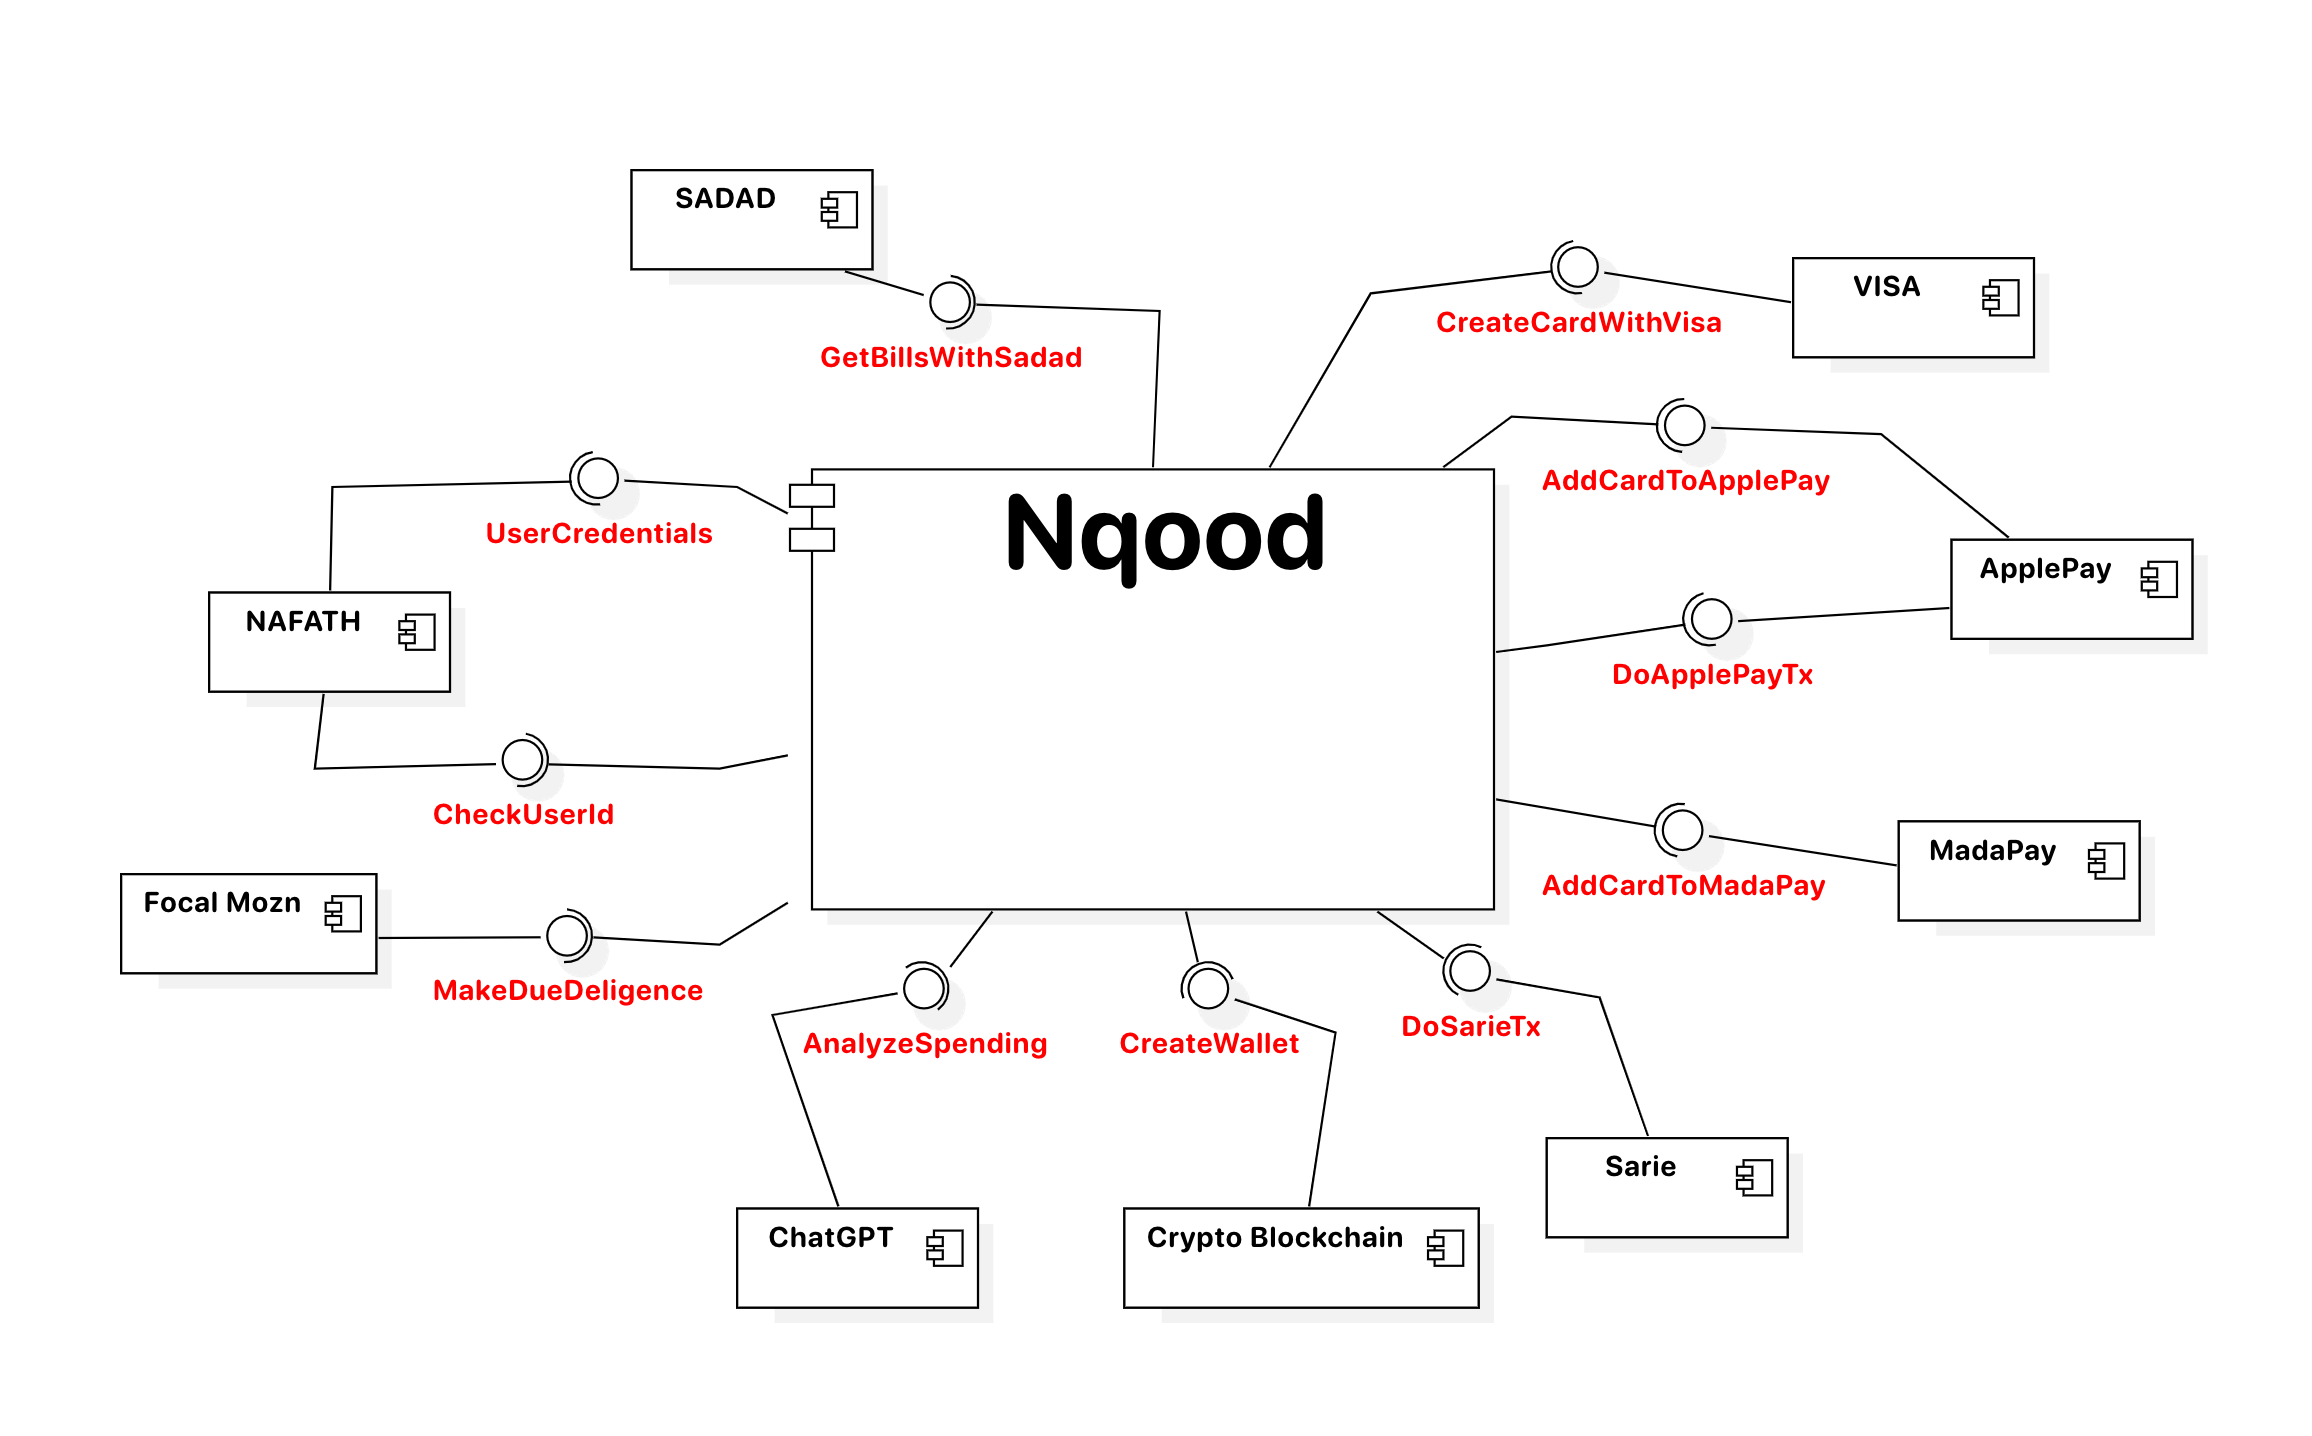
\includegraphics[width=0.8\textwidth]{images/nqood-big-picture.png}
    \caption{Nqood Big Picture}
    \label{fig:big-picture}
\end{figure}

Figure \ref{fig:big-picture} elaborates how the Nqood system communicates with all the external systems. It shows how the frontend receives the information from the backend which collects it from different sources.

\chapter{Black Box}

\begin{figure}[h!]
    \centering
    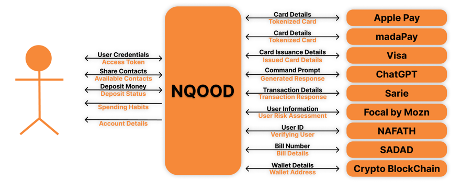
\includegraphics[width=0.8\textwidth]{images/nqood-black-box.png}
    \caption{Nqood Black Box}
    \label{fig:black-box}
\end{figure}

Figure \ref{fig:black-box} demonstrates all the possible inputs and outputs of both a Nqood user and the external systems. Below is a more detailed description of each input/output combination:

\chapter{Design Package Diagram}

\begin{figure}[h!]
    \centering
    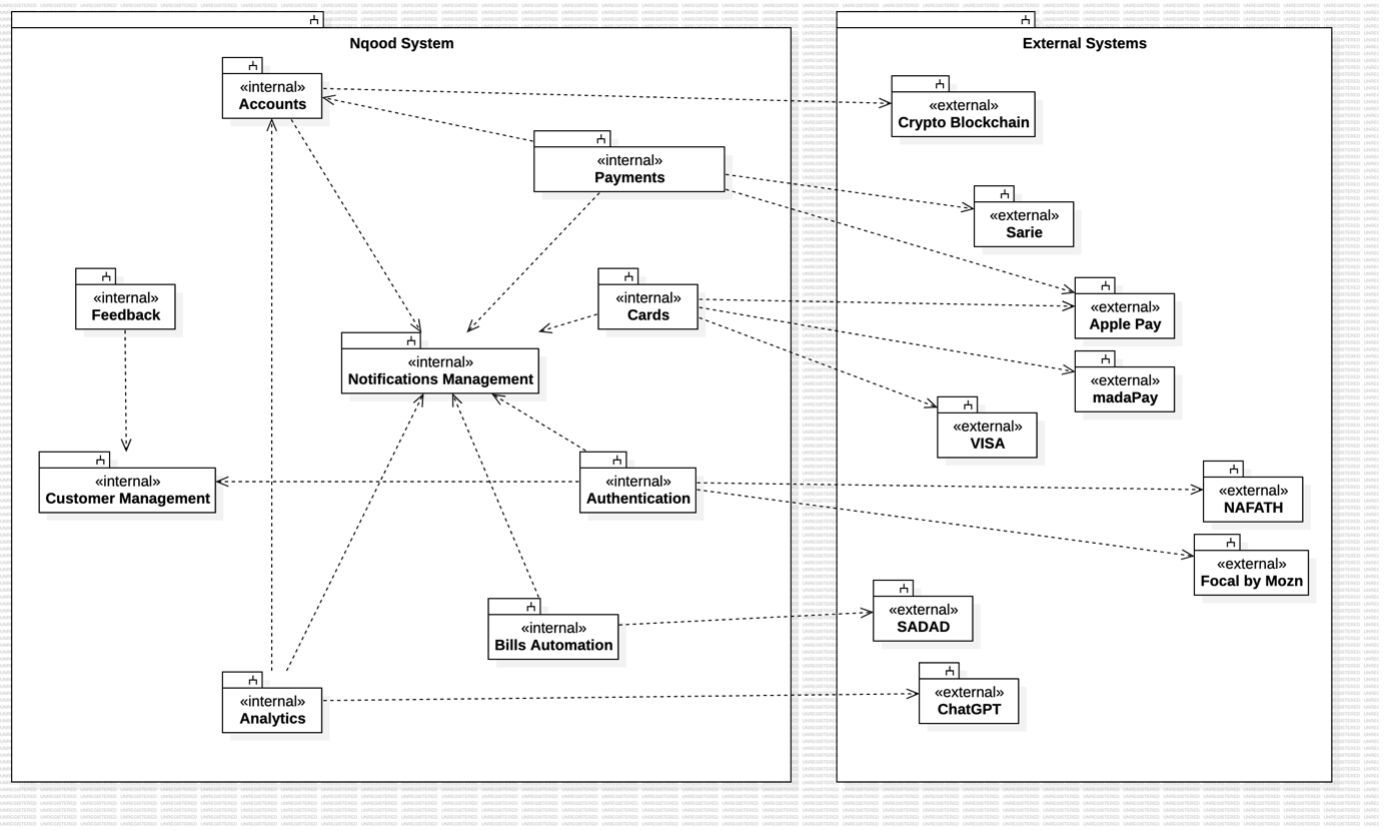
\includegraphics[width=0.8\textwidth]{images/nqood-package-diagram.png}
    \caption{Nqood Package Diagram}
    \label{fig:package-diagram}
\end{figure}

Figure \ref{fig:package-diagram} illustrates how the Nqood system has many external dependencies managed by internal subsystems that make the wallet functionality possible.

Each internal subsystem in the Nqood system has its own database to make each subsystem independent. Below is a description of the 9 internal subsystems:

\chapter{Nqood Methodology}

\begin{figure}[h!]
    \centering
    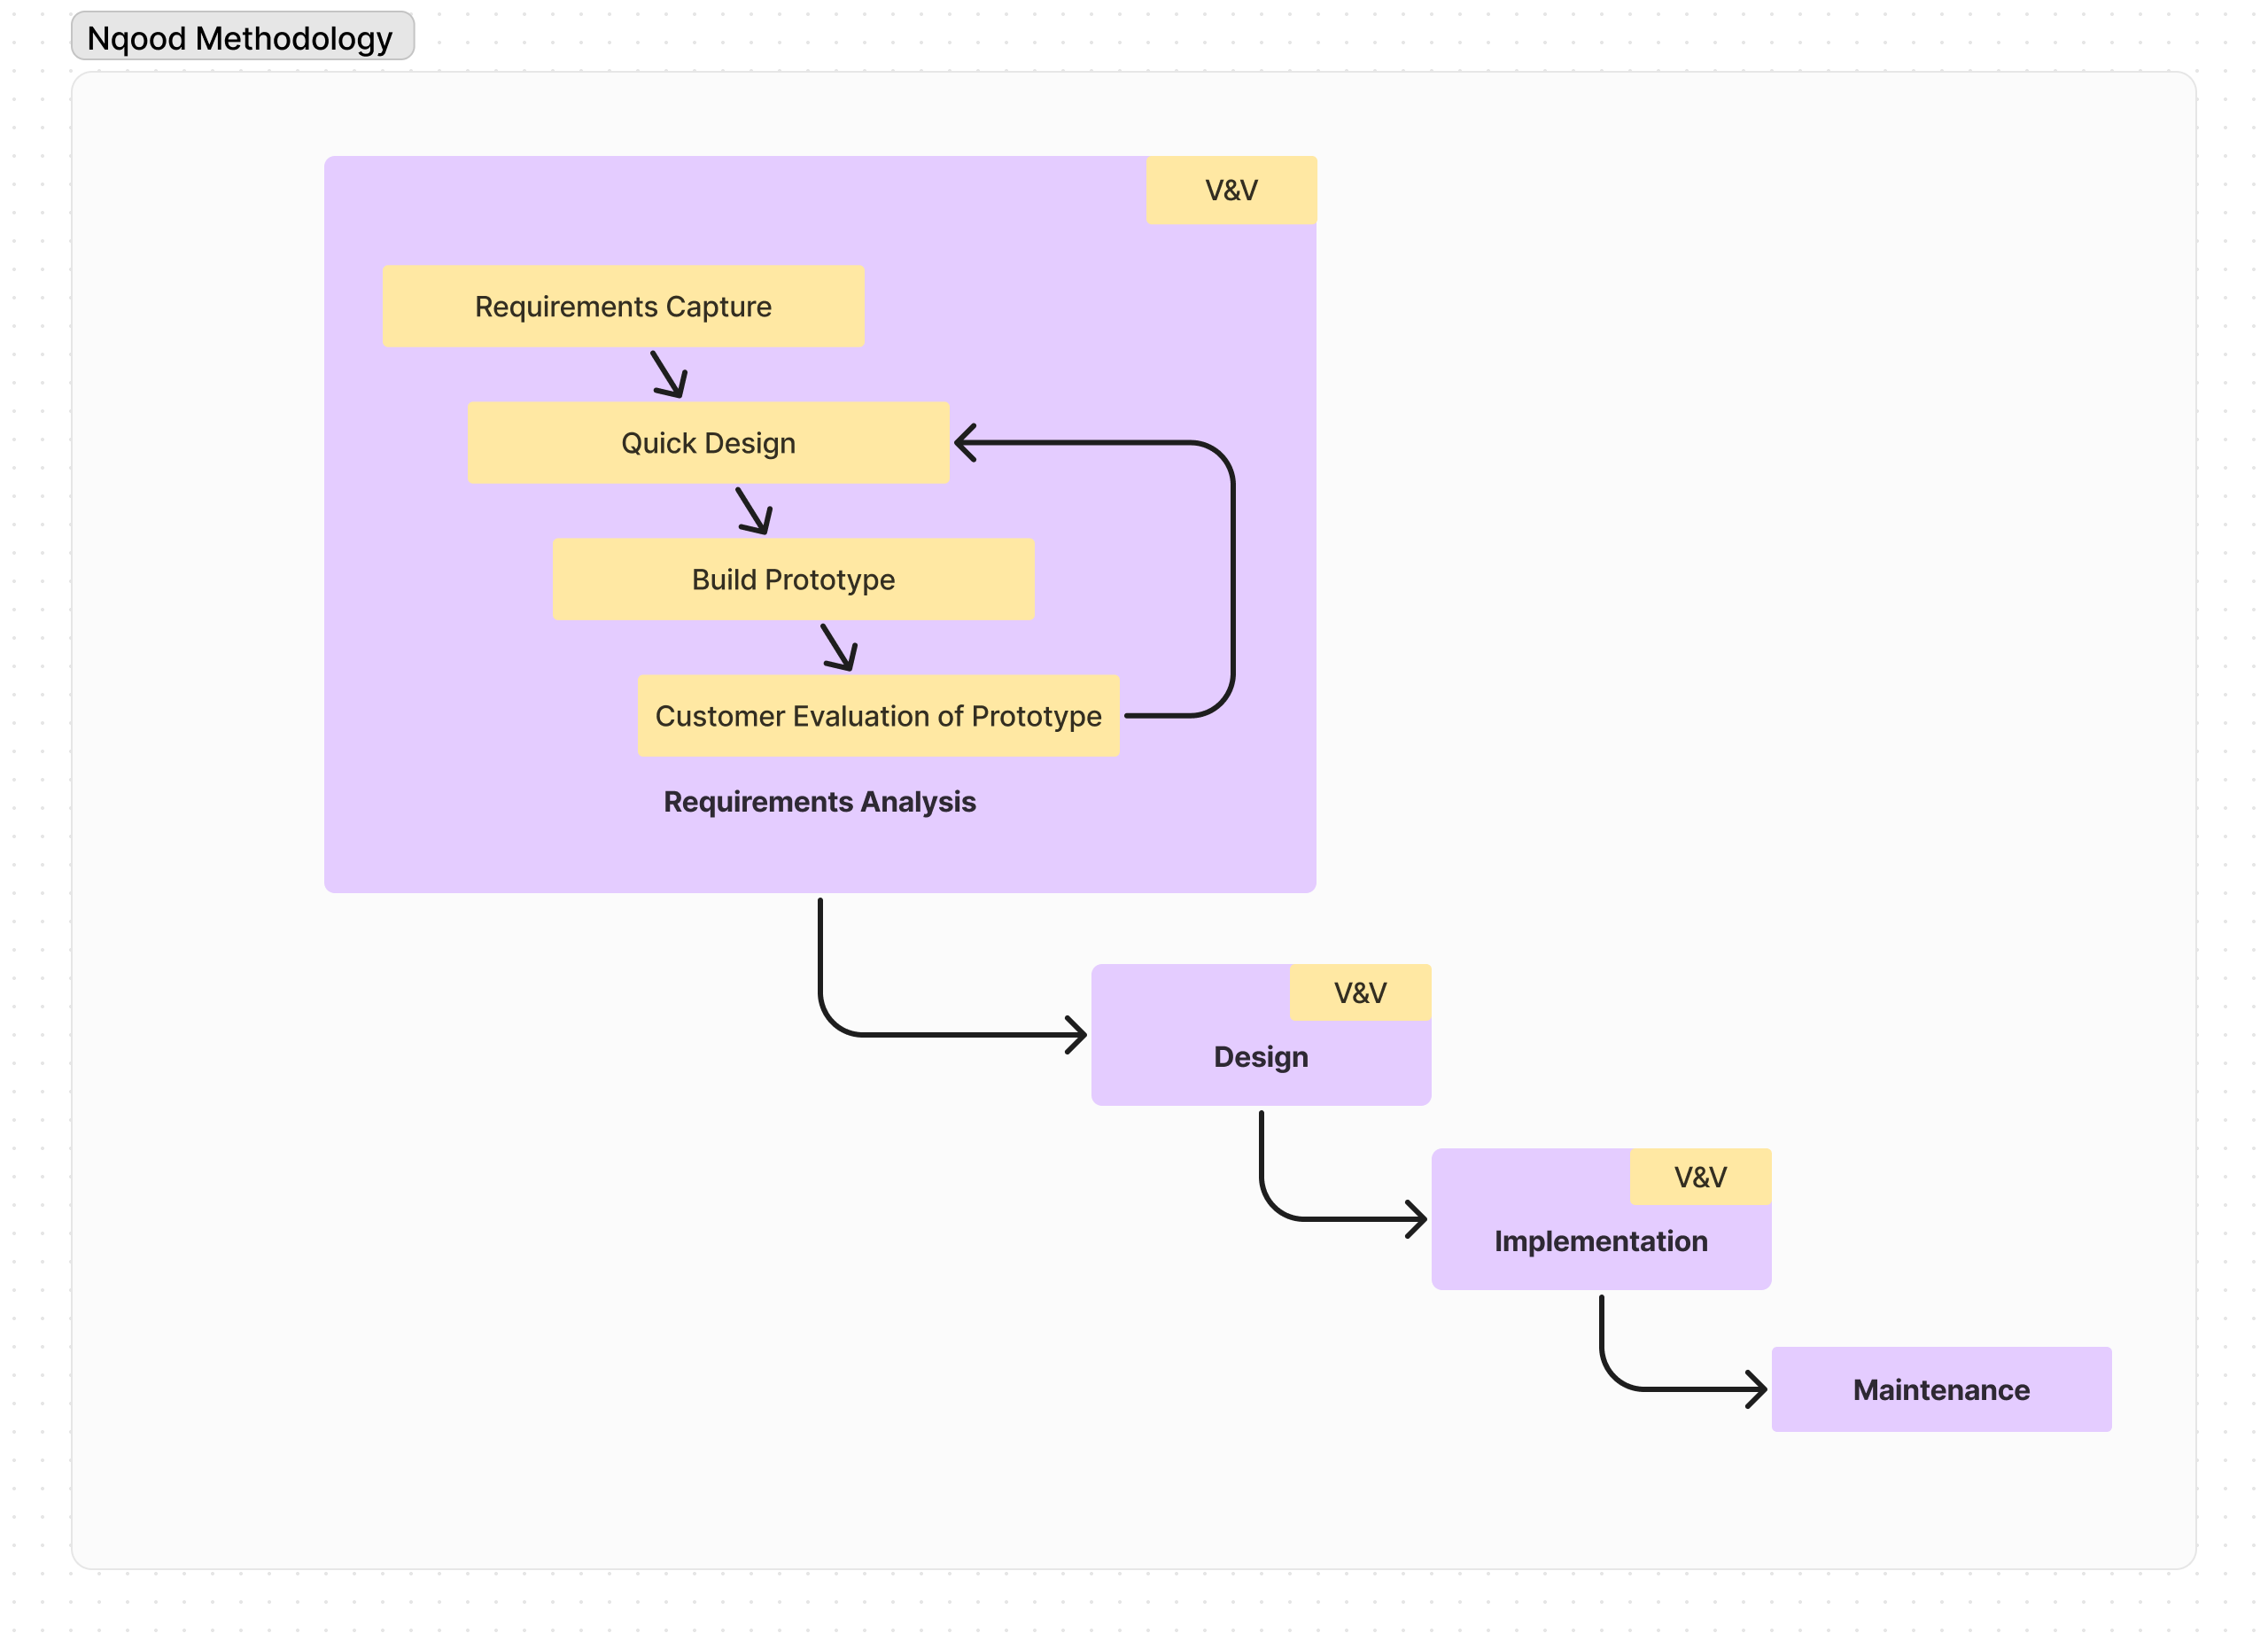
\includegraphics[width=0.8\textwidth]{images/nqood-methodology.png}
    \caption{Nqood Methodology}
    \label{fig:nqood-methodology}
\end{figure}

We chose the waterfall model. In industries with strict regularity compliance the waterfall's
document focused approach can be beneficial. It insures that all requirements are documented, implemented and tested
throughly. 

We injected prototyping in the requirements phase because we have complex requirements. Waterfall is the best methodology if there are well-defined requirements.

And in every phase we added a V\&V stage. We care a lot about Quality. Quality is important when building a secure and elegant digital wallet. If we don't bake the quality in, we won't have a great product!

\end{document}
